\documentclass[]{report}
\usepackage{lmodern}
\usepackage{amssymb,amsmath}
\usepackage{ifxetex,ifluatex}
\usepackage{fixltx2e} % provides \textsubscript
\ifnum 0\ifxetex 1\fi\ifluatex 1\fi=0 % if pdftex
  \usepackage[T1]{fontenc}
  \usepackage[utf8]{inputenc}
\else % if luatex or xelatex
  \ifxetex
    \usepackage{mathspec}
  \else
    \usepackage{fontspec}
  \fi
  \defaultfontfeatures{Ligatures=TeX,Scale=MatchLowercase}
\fi
% use upquote if available, for straight quotes in verbatim environments
\IfFileExists{upquote.sty}{\usepackage{upquote}}{}
% use microtype if available
\IfFileExists{microtype.sty}{%
\usepackage{microtype}
\UseMicrotypeSet[protrusion]{basicmath} % disable protrusion for tt fonts
}{}
\usepackage{hyperref}
\hypersetup{unicode=true,
            pdftitle={DATA 624: Project 2},
            pdfauthor={Vinicio Haro; Sang Yoon (Andy) Hwang; Julian McEachern; Jeremy O'Brien; Bethany Poulin},
            pdfborder={0 0 0},
            breaklinks=true}
\urlstyle{same}  % don't use monospace font for urls
\usepackage{color}
\usepackage{fancyvrb}
\newcommand{\VerbBar}{|}
\newcommand{\VERB}{\Verb[commandchars=\\\{\}]}
\DefineVerbatimEnvironment{Highlighting}{Verbatim}{commandchars=\\\{\}}
% Add ',fontsize=\small' for more characters per line
\usepackage{framed}
\definecolor{shadecolor}{RGB}{248,248,248}
\newenvironment{Shaded}{\begin{snugshade}}{\end{snugshade}}
\newcommand{\AlertTok}[1]{\textcolor[rgb]{0.94,0.16,0.16}{#1}}
\newcommand{\AnnotationTok}[1]{\textcolor[rgb]{0.56,0.35,0.01}{\textbf{\textit{#1}}}}
\newcommand{\AttributeTok}[1]{\textcolor[rgb]{0.77,0.63,0.00}{#1}}
\newcommand{\BaseNTok}[1]{\textcolor[rgb]{0.00,0.00,0.81}{#1}}
\newcommand{\BuiltInTok}[1]{#1}
\newcommand{\CharTok}[1]{\textcolor[rgb]{0.31,0.60,0.02}{#1}}
\newcommand{\CommentTok}[1]{\textcolor[rgb]{0.56,0.35,0.01}{\textit{#1}}}
\newcommand{\CommentVarTok}[1]{\textcolor[rgb]{0.56,0.35,0.01}{\textbf{\textit{#1}}}}
\newcommand{\ConstantTok}[1]{\textcolor[rgb]{0.00,0.00,0.00}{#1}}
\newcommand{\ControlFlowTok}[1]{\textcolor[rgb]{0.13,0.29,0.53}{\textbf{#1}}}
\newcommand{\DataTypeTok}[1]{\textcolor[rgb]{0.13,0.29,0.53}{#1}}
\newcommand{\DecValTok}[1]{\textcolor[rgb]{0.00,0.00,0.81}{#1}}
\newcommand{\DocumentationTok}[1]{\textcolor[rgb]{0.56,0.35,0.01}{\textbf{\textit{#1}}}}
\newcommand{\ErrorTok}[1]{\textcolor[rgb]{0.64,0.00,0.00}{\textbf{#1}}}
\newcommand{\ExtensionTok}[1]{#1}
\newcommand{\FloatTok}[1]{\textcolor[rgb]{0.00,0.00,0.81}{#1}}
\newcommand{\FunctionTok}[1]{\textcolor[rgb]{0.00,0.00,0.00}{#1}}
\newcommand{\ImportTok}[1]{#1}
\newcommand{\InformationTok}[1]{\textcolor[rgb]{0.56,0.35,0.01}{\textbf{\textit{#1}}}}
\newcommand{\KeywordTok}[1]{\textcolor[rgb]{0.13,0.29,0.53}{\textbf{#1}}}
\newcommand{\NormalTok}[1]{#1}
\newcommand{\OperatorTok}[1]{\textcolor[rgb]{0.81,0.36,0.00}{\textbf{#1}}}
\newcommand{\OtherTok}[1]{\textcolor[rgb]{0.56,0.35,0.01}{#1}}
\newcommand{\PreprocessorTok}[1]{\textcolor[rgb]{0.56,0.35,0.01}{\textit{#1}}}
\newcommand{\RegionMarkerTok}[1]{#1}
\newcommand{\SpecialCharTok}[1]{\textcolor[rgb]{0.00,0.00,0.00}{#1}}
\newcommand{\SpecialStringTok}[1]{\textcolor[rgb]{0.31,0.60,0.02}{#1}}
\newcommand{\StringTok}[1]{\textcolor[rgb]{0.31,0.60,0.02}{#1}}
\newcommand{\VariableTok}[1]{\textcolor[rgb]{0.00,0.00,0.00}{#1}}
\newcommand{\VerbatimStringTok}[1]{\textcolor[rgb]{0.31,0.60,0.02}{#1}}
\newcommand{\WarningTok}[1]{\textcolor[rgb]{0.56,0.35,0.01}{\textbf{\textit{#1}}}}
\usepackage{graphicx,grffile}
\makeatletter
\def\maxwidth{\ifdim\Gin@nat@width>\linewidth\linewidth\else\Gin@nat@width\fi}
\def\maxheight{\ifdim\Gin@nat@height>\textheight\textheight\else\Gin@nat@height\fi}
\makeatother
% Scale images if necessary, so that they will not overflow the page
% margins by default, and it is still possible to overwrite the defaults
% using explicit options in \includegraphics[width, height, ...]{}
\setkeys{Gin}{width=\maxwidth,height=\maxheight,keepaspectratio}
\IfFileExists{parskip.sty}{%
\usepackage{parskip}
}{% else
\setlength{\parindent}{0pt}
\setlength{\parskip}{6pt plus 2pt minus 1pt}
}
\setlength{\emergencystretch}{3em}  % prevent overfull lines
\providecommand{\tightlist}{%
  \setlength{\itemsep}{0pt}\setlength{\parskip}{0pt}}
\setcounter{secnumdepth}{0}

%%% Use protect on footnotes to avoid problems with footnotes in titles
\let\rmarkdownfootnote\footnote%
\def\footnote{\protect\rmarkdownfootnote}

%%% Change title format to be more compact
\usepackage{titling}

% Create subtitle command for use in maketitle
\providecommand{\subtitle}[1]{
  \posttitle{
    \begin{center}\large#1\end{center}
    }
}

\setlength{\droptitle}{-2em}

  \title{DATA 624: Project 2}
    \pretitle{\vspace{\droptitle}\centering\huge}
  \posttitle{\par}
    \author{Vinicio Haro \\ Sang Yoon (Andy) Hwang \\ Julian McEachern \\ Jeremy O'Brien \\ Bethany Poulin}
    \preauthor{\centering\large\emph}
  \postauthor{\par}
      \predate{\centering\large\emph}
  \postdate{\par}
    \date{10 December 2019}

% set plain style for page numbers
\usepackage[margin=1in]{geometry}
\usepackage{fancyhdr}
\pagestyle{fancy}
\fancyhead[LE,RO]{\textbf{Group 2}}
\fancyhead[RE,LO]{\textbf{Project 2: Predicting PH}}
\raggedbottom
\setlength{\parskip}{1em}

% change font
\usepackage{fontspec}
\setmainfont{Arial}

% format titles 
\usepackage{xcolor}
\usepackage{sectsty}
\usepackage{etoolbox}
\usepackage{titling}
\definecolor{prettyblue}{RGB}{84, 144, 240}
\definecolor{bluegray}{RGB}{98, 107, 115}
\pretitle{\begin{center}\Huge\color{prettyblue}\textbf}
\posttitle{\par\LARGE\color{gray}DATA 624 - Predictive Analytics\linebreak Group 2\end{center}}
\preauthor{\begin{center}\large\textbf{Group Members:}\linebreak\textit}
\postauthor{\end{center}}

% Format chapter output
\usepackage{titlesec}
\titleclass{\part}{top}
\titleclass{\chapter}{straight}
\titleformat{\chapter}
  {\normalfont\color{prettyblue}\LARGE\bfseries}{\thechapter}{1em}{}
\titlespacing*{\chapter}{0pt}{3.5ex plus 1ex minus .2ex}{2.3ex plus .2ex}


% create color block quotes
\usepackage{tcolorbox}
\newtcolorbox{myquote}{colback=purple!05!white, colframe=purple!75!black}
\renewenvironment{quote}{\begin{myquote}}{\end{myquote}}

% kable 
\usepackage{tabu}


% multicolumn
\usepackage{multicol}

% bullets
\newenvironment{tight_enumerate}{
\begin{enumerate}
  \setlength{\itemsep}{0pt}
  \setlength{\parskip}{0pt}
  }{\end{enumerate}}
  
\newenvironment{tight_itemize}{
\begin{itemize}
  \setlength{\topsep}{0pt}
  \setlength{\itemsep}{0pt}
  \setlength{\parskip}{0pt}
  \setlength{\parsep}{0pt}
  }{\end{itemize}}

\usepackage{paralist}

%hyperlink
\usepackage{hyperref}
\hypersetup{
    colorlinks=true,
    linkcolor=bluegray,
    filecolor=magenta,      
    urlcolor=cyan}

\usepackage{graphicx}
\usepackage{wrapfig}
\usepackage{booktabs}
\definecolor{yale}{RGB}{13,77,146}
\usepackage[font={color=yale,bf,scriptsize},figurename=Fig.,belowskip=0pt,aboveskip=0pt]{caption}
\usepackage{floatrow}
\floatsetup[figure]{capposition=above}
\floatsetup[table]{capposition=above}
\setlength{\abovecaptionskip}{1pt}
\setlength{\belowcaptionskip}{1pt}
\setlength{\textfloatsep}{2pt plus 0.5pt minus 0.5pt}
\setlength{\intextsep}{2pt plus 0.5pt minus 0.5pt}
\usepackage{booktabs}
\usepackage{longtable}
\usepackage{array}
\usepackage{multirow}
\usepackage{wrapfig}
\usepackage{float}
\usepackage{colortbl}
\usepackage{pdflscape}
\usepackage{tabu}
\usepackage{threeparttable}
\usepackage{threeparttablex}
\usepackage[normalem]{ulem}
\usepackage{makecell}
\usepackage{xcolor}

\begin{document}
\maketitle

{
\setcounter{tocdepth}{1}
\tableofcontents
}
File for final submission of Project 2.

\thispagestyle{empty}
\newpage
\clearpage
\pagenumbering{arabic}

\hypertarget{executive-summary}{%
\chapter{Executive Summary}\label{executive-summary}}

Because it is to central to the design of a product's drinking
experience, pH is a key performance indicator in the beverage
manufacturing process and is tested for and tracked diligently, as the
final pH is dependent on and vulnerable to even slight changes in
production methods.

Having monitored and recorded these production variables, as well as the
final pH, we have the opportunity to improve production outcomes by more
closely controlling pH in our beverages with predictive modeling with
the potential to catch and correct variations in process which negative
impact our taget pH.

{[}CONTENT EDITORS: ADD IN SUMMARY OF CONCLUSION AND ANY SUPPORTING
INSIGHT FROM LAST SECTION{]}

\hypertarget{approach}{%
\chapter{Approach}\label{approach}}

After thorough examination, we approached this task by splitting the
provided data into training and test sets. We evaluated several models
on this split and found that \textbf{what-ever-worked-best} method
yielded the best results.

Each group member worked individually to create their own solution. We
built our final submission by collaboratively evaluating and combining
each others' approaches.

{[}CONTENT EDITORS: ADD IN FOLLOWING LAST: Our introduction should
further outline individual responsibilities. For example,
\textbf{so-and-so} was responsible for \textbf{xyz task}.{]}

{[}FORMAT EDITORS: UPDATE BELOW{]} For replication and grading purposes,
we made our code avaliable in the appendix section. This code, along
with the provided data, score-set results, and individual contributions,
can also be accessed through our group github repository:

\begin{compactitem}
  \item \href{https://github.com/JeremyOBrien16/CUNY_DATA_624/tree/master/Project_Two}{Pretend I'm a working link to R Source Code}
  \item \href{https://github.com/JeremyOBrien16/CUNY_DATA_624/tree/master/Project_Two}{Pretend I'm a working link to Provided Data}
  \item \href{https://github.com/JeremyOBrien16/CUNY_DATA_624/tree/master/Project_Two}{Pretend I'm a working link to Excel Results}
  \item \href{https://github.com/JeremyOBrien16/CUNY_DATA_624/tree/master/Project_Two}{Pretend I'm a working link to Individual Work}
\end{compactitem}

\hypertarget{data-exploration}{%
\chapter{Data Exploration}\label{data-exploration}}

Preparing the data was the most discussed and influential part of our
modeling process. It was clear from early on that in order to build a
useful model with such a narrow range of expected pH values, how we
groomed our data and the decisions we made would likely be as or more
influential than the model we ultimately chose.

The beverage dataset includes 2,571 cases, 32 predictor variables, and a
single response variable. One of these predictor variables (Brand Code)
is categorical with four levels - A through D; for the purpose of our
analysis we interpreted these to represent four distinct beverage
brands.

While we found missing observations in both response and predictor
variables, in our assessment the extent of NAs did not suggest a
systemic issue in measurement or recording that imputing values could
not remedy. For context: - The response variable (PH) is missing a total
of four observations (\textless{} 1\%). - Most (30) predictor variables
are missing at least one observation, but only eleven are missing more
than 1\% of total cases and only three are missing more than 2\% of
total cases. These are: 1. MFR (continuous, 8.2\%) 2. BrandCode
(categorical, 4.7\%) 3. and FillerSpeed (continuous, 2.2\%)

{[}CONTENT EDITORS: DO WE STILL WANT TO CREATE MISSING DATA TABLE? IF
SO, MISSINGDATA OBJECT NEEDS TO BE REBUILT IN MODEL\_PREP.R{]}

\begin{table}[H]

\caption{\label{tab:unnamed-chunk-2}Variables with Highest Frequency of NA Values}
\centering
\fontsize{8}{10}\selectfont
\begin{tabular}{lrrrrrrrrrrr}
\toprule
\textbf{ } & \textbf{MFR} & \textbf{BrandCode} & \textbf{FillerSpeed} & \textbf{PCVolume} & \textbf{PSCCO2} & \textbf{FillOunces} & \textbf{PSC} & \textbf{CarbPressure1} & \textbf{HydPressure4} & \textbf{CarbPressure} & \textbf{CarbTemp}\\
\midrule
\rowcolor{gray!6}  n & 212.0 & 120.0 & 57.0 & 39.0 & 39.0 & 38.0 & 33.0 & 32.0 & 30.0 & 27.0 & 26\\
\% & 8.2 & 4.7 & 2.2 & 1.5 & 1.5 & 1.5 & 1.3 & 1.2 & 1.2 & 1.1 & 1\\
\bottomrule
\end{tabular}
\end{table}

\hypertarget{response-variable}{%
\section{Response Variable}\label{response-variable}}

{[}CONTENT EDITORS: DO WE STILL WANT TO CREATE VARIABLE HISTOGRAMS?{]}

\begin{wrapfigure}{r}{0.5\textwidth}

\hfill{}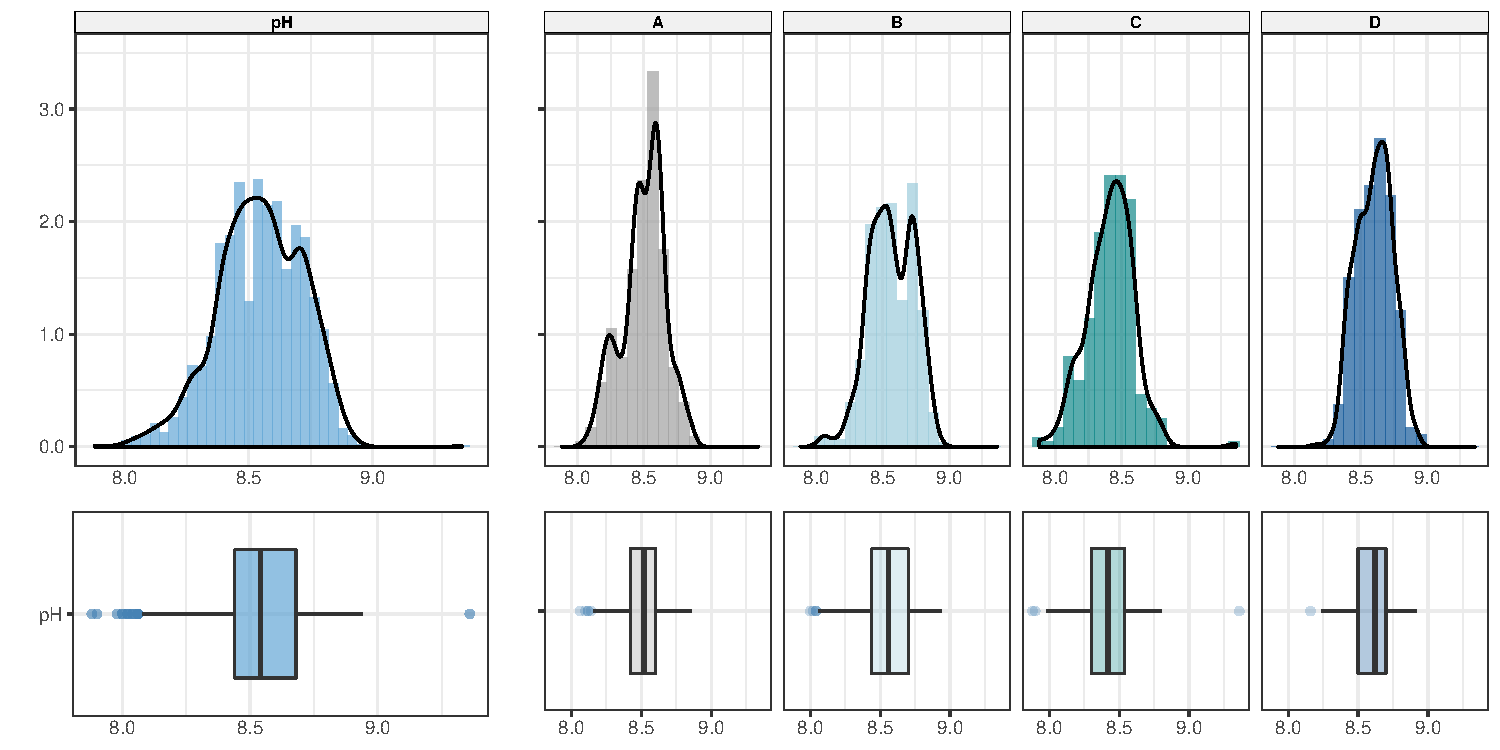
\includegraphics[width=1\textwidth]{CONFLICT_Project_Update_files/figure-latex/unnamed-chunk-3-1} 

\caption{Distribution of Response Variable: pH}\label{fig:unnamed-chunk-3}
\end{wrapfigure}

The response variable PH is a logarithmically scaled measure of how
acidic or basic a water-based solution is
(\url{https://en.wikipedia.org/wiki/PH}). It ranges from 0 (acidic) and
to 14 (alkaline); 7 is neutral (e.g.~room temperature water).

In aggregate, PH distribution is approximately normal and centered
around 8.546 (i.e.~slightly base), with some negative skew / outliers.
When evaluated by BrandCode: - A (293 observations) appears to be
multimodal and have the most outliers, with a mean slightly lower than
the aggregate (8.495) - B (1293 observations) appears to be bimodal with
a number of outliers, as well as a mean nearest the aggregate (8.562) -
C (304 observations) appears to be bimodal and is the most acid (8.419)
- D (615 observations) is the most normal distribution and also has the
highest alkalinity (8.603)

\hypertarget{predictor-variables}{%
\section{Predictor Variables}\label{predictor-variables}}

We examined the density of our variables to visualize the distribution
of the predictors. Many of these variables contain outliers and present
with a skewed distribution. The outliers fall outside the red-line
boundaries, and highlight which predictors have heavier tails.

The density plots also contain an overlay of the only categorical
indicator, \texttt{BrandCode}. This view shows us that some variables,
including \texttt{AlchRel}, \texttt{CarbRel}, \texttt{CarbVolume},
\texttt{HydPressure4}, and \texttt{Tempature}, are strongly influenced
by brand type.

{[}CONTENT EDITORS: DO WE STILL WANT TO CREATE THESE TABLES? IF SO,
OUTLIER\_WITH OBJECT NEEDS TO BE REBUILT IN MODEL\_PREP.R{]}

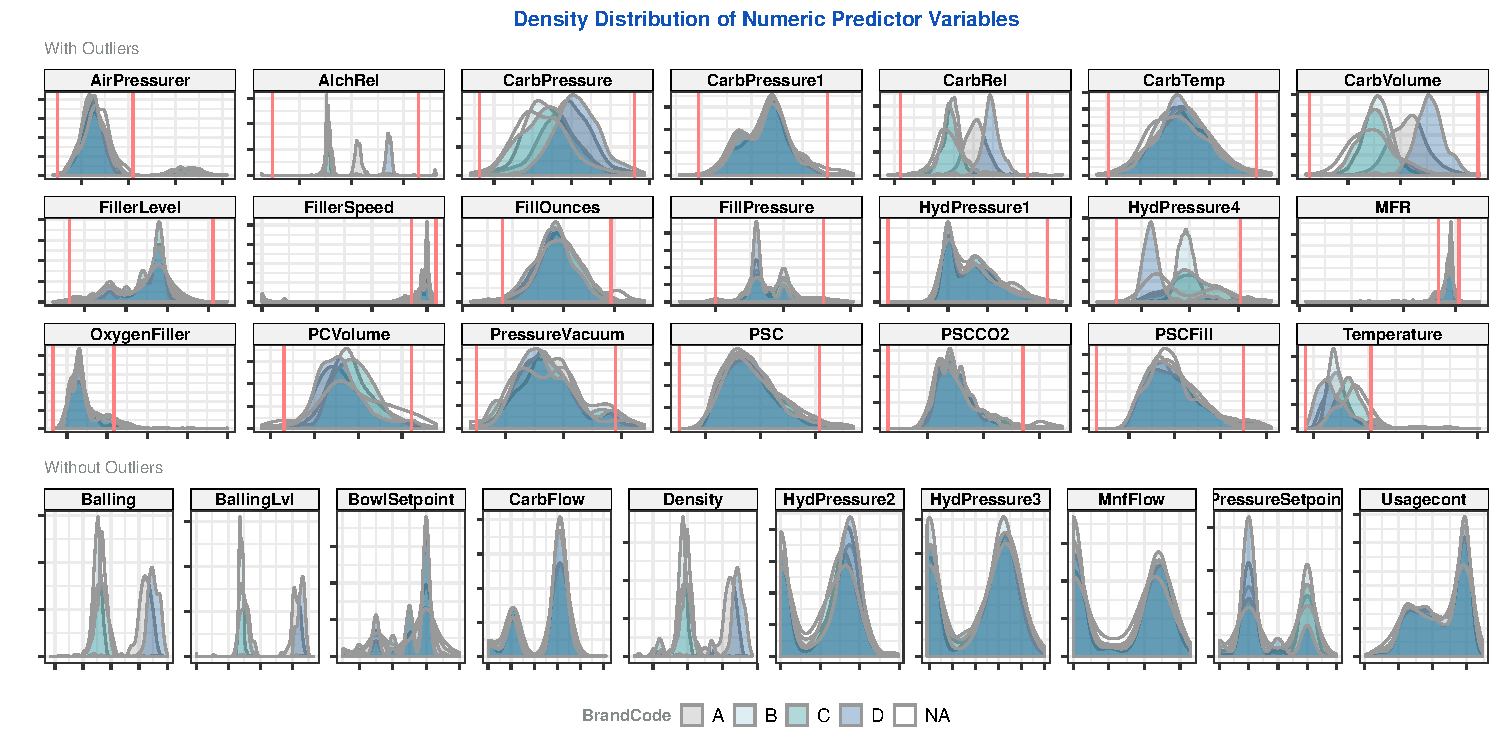
\includegraphics{CONFLICT_Project_Update_files/figure-latex/unnamed-chunk-4-1.pdf}

As no predictor variable shows a particularly pronounced monotonic
linear relationship with response, a non-linear approach to modeling
seems warranted.

{[}FIGURE SUCH AND SUCH{]} helps to further visualize the effect
\texttt{BrandCode} has on our predictor and \texttt{pH} values. For
example, \texttt{AlchRel} shows distinct \texttt{BrandCode} groupings.
Other variables, such as \texttt{PSCO2}, \texttt{BowlSetpoint},
\texttt{MinFlow}, and \texttt{PressureSetup} show unique features likely
related to system processes.

{[}CONTENT EDITORS: DO WE STILL WANT TO CREATE THESE TABLES? IF SO,
OUTLIER\_WITH OBJECT NEEDS TO BE REBUILT IN MODEL\_PREP.R{]}

** Leaving scatter plts for now. Suggestion - maybe trunicate to the the
top \emph{X} correlated with pH or incorporate after varImp for final
modes - Or just delete if too cluttered **

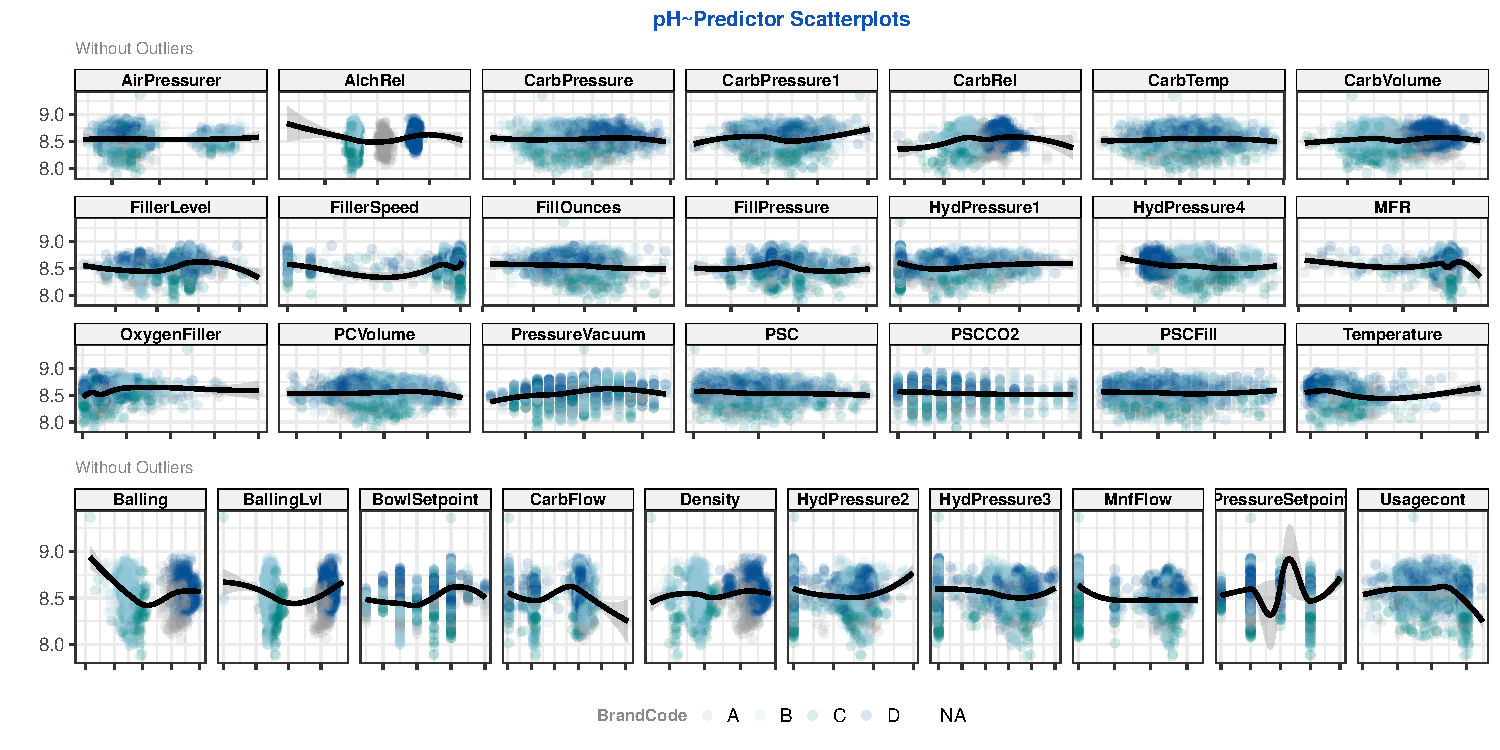
\includegraphics{CONFLICT_Project_Update_files/figure-latex/unnamed-chunk-5-1.pdf}

Collinearity measures between numeric predictors indicate that several
of these variables are heavily related, with correlation values
exceeding \(\pm{0.7}\).

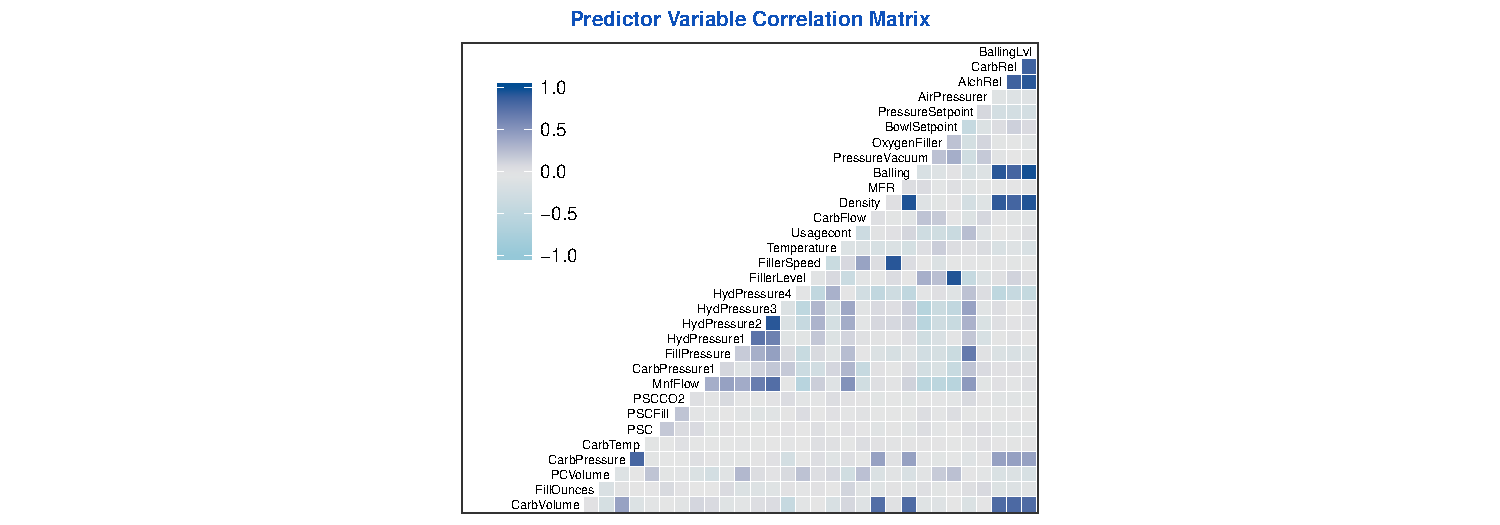
\includegraphics{CONFLICT_Project_Update_files/figure-latex/unnamed-chunk-6-1.pdf}

\hypertarget{data-preparation}{%
\chapter{Data Preparation}\label{data-preparation}}

In our exploration, we detected missing data, extreme outliers, and
multicollinearity. We kept these factors in mind and applied strategic
transformations when preparing our models to evaluate their performance
with and without normalization changes.

\textbf{Train/Test Splits:}

Prior to all pre-processing, we divided the production dataset using an
80/20 split to create a train and test sets.

{[}BETHANY / JULIANN: PLEASE CONFIRM THIS IS STILL ACCURATE:

All models incorporated k-folds cross-validation set at 10 folds to
protect against overfitting the data. We set up unique model tuning
grids to find the optimal parameters for each regression type to ensure
the highest accuracy within our predictions.

For both KNN and SVM models a grid of seeds was created from our
original seed to ensure that out repeated cross validation would be
repeateable. The same seeds were used in both the SVM and KNN.

{]}

\textbf{Data Imputation:}

Missing values are imputed using the \texttt{caret} package so that the
same range of imputed values could be applied to the test and validation
sets without confounding our training data and a bagging algorithm was
used to impute all continuous variables.

Because we were convinced that the 'brand variable \texttt{BrandCode}
may be one of the strongest predictors of pH, after much discussion, we
decided not to impute the Brand Code variable, so that each of the
observations with a known brand would be more accurately described by
the other variables relative to pH.

Instead the missing labels were replaces with Unknown and the variables
were converted to dummies of 0 and 1 to ensure that all modeling methods
would be able to consider Brand Code.

Test data is imputed with the same model, with that target variable
\texttt{PH} removed from the set.

\textbf{Pre-Processing:}

Most of the models concidered in our modeling process require scaling
and centering, so we included this in our prepartions. Although, only
one variable showed near-zero variance, Hyde.Pressure\_1 we opted to
remove it from all models during preprocessing and likewise applied
Box-Cox conversions to the data to compensate for andy skews and
non-normal modaliteis in the variables which might confound our models.
Again, the preprocessing model was saved so that the test and validation
sets could be consistenly transformed using caret's predict method.

\hypertarget{modeling}{%
\chapter{Modeling}\label{modeling}}

We assessed the effectiveness of more than ten different non-linear
regression models in our exploratory process. We settled on four models
that exhibited the most favorable test metrics, tuned those models, and
then chose the best performing model of that set to use in our final
analyses (all performance results from the other five are included in
{[}TABLE BLAH BLAH{]} in {[}APPENDIX BLAH BLAH{]}).

{[}BETHANY: INSERT SIDE-BY-SIDE TRAINING / TESTING METRICS FOR
PREPRCESSED MODELS (SET 2) HERE{]}.

\begin{itemize}
\tightlist
\item
  Model 1: Support Vector Machines Regression
\item
  Model 2: Cubist Tree Regression
\item
  Model 3: Multivariate Adaptive Regression Splines Regression
\item
  Model 4: Random Forest Regression
\end{itemize}

\hypertarget{model-performance}{%
\chapter{Model Performance}\label{model-performance}}

\begin{itemize}
\tightlist
\item
  Set1 = Caret: bagImputed; no additional pre-processing\\
\item
  Set2 = Caret: bagImputed; PreP
  \texttt{method=c(\textquotesingle{}center\textquotesingle{},\ \textquotesingle{}scale\textquotesingle{},\ \textquotesingle{}nzv\textquotesingle{},\ \textquotesingle{}BoxCox\textquotesingle{})}
\end{itemize}

\textbf{Train Performance:}

\begin{table}[H]

\caption{\label{tab:unnamed-chunk-7}Train1 Performance}
\centering
\fontsize{8}{10}\selectfont
\begin{tabular}{rrrrl}
\toprule
MAPE & RMSE & RSquared & MAE & Method\\
\midrule
\rowcolor{gray!6}  0.0079 & 0.0947 & 0.7005 & 0.0669 & cubist\\
0.0082 & 0.0973 & 0.6989 & 0.0700 & rf\\
\rowcolor{gray!6}  0.0103 & 0.1211 & 0.5144 & 0.0878 & svmRadial\\
0.0108 & 0.1226 & 0.5030 & 0.0920 & earth\\
\bottomrule
\end{tabular}
\end{table}

\begin{table}[H]

\caption{\label{tab:unnamed-chunk-7}Train2 Performance}
\centering
\fontsize{8}{10}\selectfont
\begin{tabular}{rrrrl}
\toprule
MAPE & RMSE & RSquared & MAE & Method\\
\midrule
\rowcolor{gray!6}  1.1928 & 0.5719 & 0.6860 & 0.4105 & rf\\
1.2637 & 0.5602 & 0.6851 & 0.3924 & cubist\\
\rowcolor{gray!6}  1.4182 & 0.6990 & 0.5139 & 0.5068 & svmRadial\\
1.6893 & 0.7166 & 0.4915 & 0.5374 & earth\\
\bottomrule
\end{tabular}
\end{table}

\textbf{Test Accuracy:}

\begin{table}[H]

\caption{\label{tab:unnamed-chunk-8}Test1 Performance}
\centering
\fontsize{8}{10}\selectfont
\begin{tabular}{rrrrl}
\toprule
MAPE & RMSE & Rsquared & MAE & Method\\
\midrule
\rowcolor{gray!6}  0.0078 & 0.0890 & 0.7254 & 0.0669 & cubist\\
0.0079 & 0.0882 & 0.7465 & 0.0670 & rf\\
\rowcolor{gray!6}  0.0101 & 0.1138 & 0.5508 & 0.0860 & svmRadial\\
NaN & 0.1246 & 0.4897 & 0.0896 & earth\\
\bottomrule
\end{tabular}
\end{table}

\begin{table}[H]

\caption{\label{tab:unnamed-chunk-8}Test2 Performance}
\centering
\fontsize{8}{10}\selectfont
\begin{tabular}{rrrrl}
\toprule
MAPE & RMSE & Rsquared & MAE & Method\\
\midrule
\rowcolor{gray!6}  1.0002 & 8.5581 & 0.5508 & 8.5364 & svmRadial\\
1.0041 & 8.5943 & 0.7286 & 8.5654 & cubist\\
\rowcolor{gray!6}  1.0043 & 8.5892 & 0.7463 & 8.5691 & rf\\
NaN & 8.6524 & 0.4645 & 8.6251 & earth\\
\bottomrule
\end{tabular}
\end{table}

{[}BETHANY: EACH OF US SHOULD WRITE BULLETS WITH REASONS TO CHOOSE THIS
MODEL BY SAT EVENING 12/7 - BETHANY WILL FLESH OUT{]}

\hypertarget{model-selection-considerations}{%
\section{Model Selection
Considerations}\label{model-selection-considerations}}

{[}BETHANY: NEED TO PICK OUR FIRST CHOICE MODEL, THINK IS SHOULD BE
VARIMP-ABLE SO WE CAN USE THAT IN INTERPRETATION / CONCLUSIONS{]}

\hypertarget{model-1-support-vector-machines-svm-regression}{%
\section{Model 1: Support Vector Machines (SVM)
Regression}\label{model-1-support-vector-machines-svm-regression}}

{[}BETHANY TO WORDSMITH RATIONALE FOR USING SVM MODEL{]}

The support vector machine, although less efficient than the k-nearest
neighbor to train, provided robust final model using a radial kernel
with a cost of 10, passed as the tune length settling on
\(\sigma = 0.020\) and \(cost = 8\) returning a \(RMSE = 0.1127\)

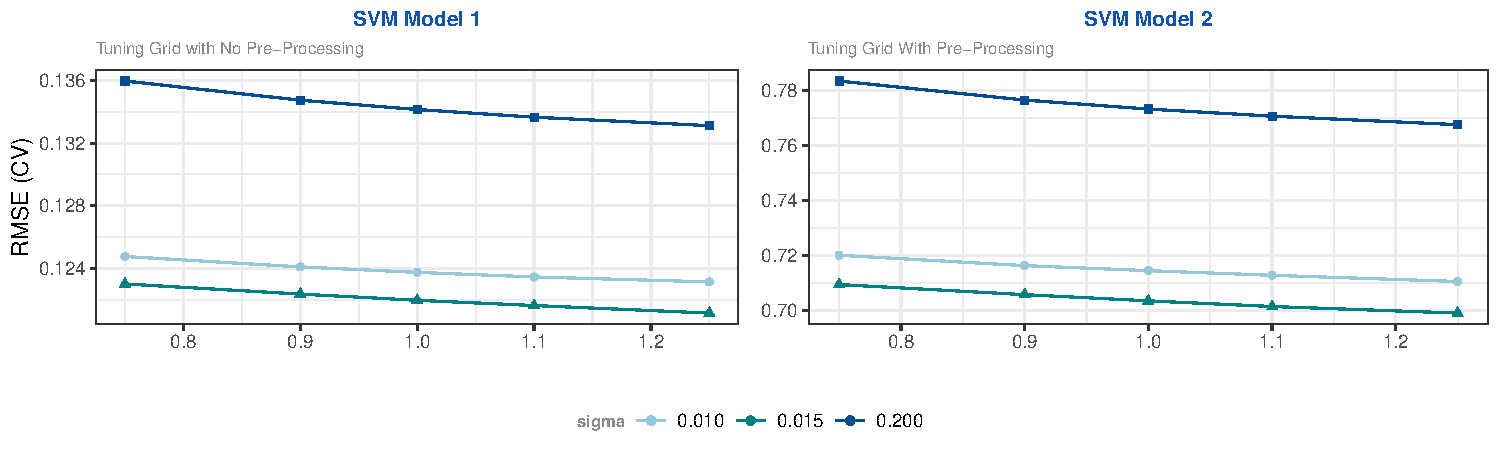
\includegraphics{CONFLICT_Project_Update_files/figure-latex/unnamed-chunk-9-1.pdf}

\hypertarget{model-2-cubist-tree-regression}{%
\section{Model 2: Cubist Tree
Regression}\label{model-2-cubist-tree-regression}}

{[}JEREMY: CONDENSING BELOW WITH RATIONALE FOR USING MODEL IN BULLET
FORM BY EVENING SAT 12/7 - BETHANY WILL WORDSMITH{]}

{[}BETHANY: PLEASE IGNORE BELOW DESCRIPTION UNTIL SAT EVENING

For a continuous response variable, a rule-based Cubist model functions
like a piecewise linear model: each rule is a conjunction of conditions
associated with a linear expression, and those rules can overlap with
each other. Adding to the interpretive complexity of those rules, Cubist
models can also integrate an instance-based, nearest-neighbor approach
that performs a composite prediction based on actual values of
neighbors, predicted values of neighbors, and predicted values of
observations of interest.

Accordingly, hyper-parameters for Cubist models include: - The number of
rule-based models, or committees - these issue separate predictions that
are averaged (5 recommended to balance computational cost with ensemble
benefits) - The number of neighbors over which to predict response
values based on similar training observations

Based on cross-validation and a grid search across hyper-parameters, we
found the best RMSE performance with an instance-based model that
factoring in many neighbors built on non-pre-processed training data.

References: Background: \url{https://www.rulequest.com/cubist-win.html}
Overview:
\url{https://static1.squarespace.com/static/51156277e4b0b8b2ffe11c00/t/56e3056a3c44d8779a61988a/1457718645593/cubist_BRUG.pdf}
Mechanics:
\url{http://ftp.uni-bayreuth.de/math/statlib/R/CRAN/doc/vignettes/caret/caretTrain.pdf}{]}

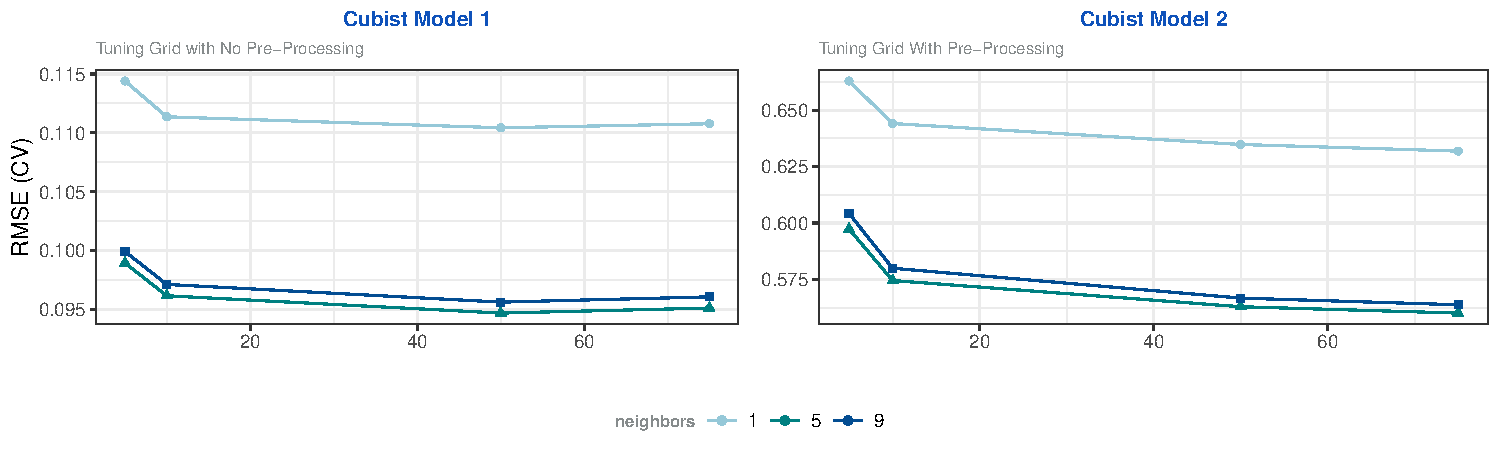
\includegraphics{CONFLICT_Project_Update_files/figure-latex/unnamed-chunk-10-1.pdf}

\hypertarget{model-3-multivariate-adaptive-regression-splines-mars-regression}{%
\section{Model 3: Multivariate Adaptive Regression Splines (MARS)
Regression}\label{model-3-multivariate-adaptive-regression-splines-mars-regression}}

{[}VINICIO / JULIANN: PLEASE ADD CONCISE BULLETS FOR USING MARS MODEL BY
EVENING SAT 12/7 - BETHANY WILL WORDSMITH{]}

MARS modeling was selected to assess the non-linear features in our
data. This method uses a weighted sum to models non-linearities and
interactions between variables. The model assesses cut-points between
features that create the smallest error and prunes insignificant points
to improve model accuracy.

Our RMSE Cross Validation plots show us that pre-processing
transformations did not have improve the MARS model. The model performed
best on our training data when no transformations were applied.

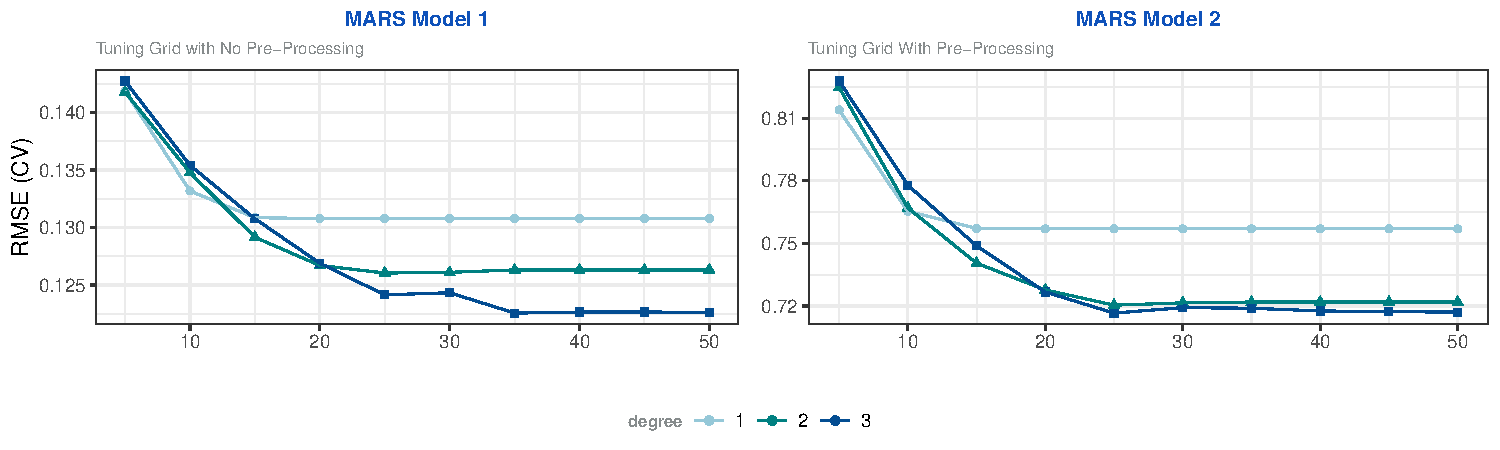
\includegraphics{CONFLICT_Project_Update_files/figure-latex/unnamed-chunk-11-1.pdf}

\hypertarget{model-4-random-forest-regression}{%
\section{Model 4: Random Forest
Regression}\label{model-4-random-forest-regression}}

{[}ANDY: PLEASE ADD CONCISE BULLETS WITH RATIONALE FOR USING RF MODEL BY
EVENING SAT 12/7 - BETHANY WILL WORDSMITH{]}

The optimal parameters for model was mtry = 31 and ntree = 2500. MAPE is
\textbf{r s\$MAPE} where as top 3 important predictors are
\texttt{MnfFlow}, \texttt{BrandCode} and \texttt{PressureVacuum} for
\%incMSE and \texttt{MnfFlow}, \texttt{BrandCode} and
\texttt{OxygenFiller} for IncNodePurity. Unlike \texttt{PLS},
\texttt{Random\ Forest} can produce 2 different variable importance
plots.

The first graph shows how much MSE would increase if a variable is
assigned with values by random permutation. The second plot is based on
\texttt{node\ purity} which is measured by the difference between RSS
before and after the split on that variable (\texttt{Gini\ Index}). In
short, each graph shows how much MSE or Impurity increases when each
variable is randomly permuted.

\begin{Shaded}
\begin{Highlighting}[]
\CommentTok{# remove echo/eval later [ANDY: ADD IN VARIMP /}
\CommentTok{# PERFORMANCE CHART FOR SVM AS ALIGNED WITH GROUP]}
\end{Highlighting}
\end{Shaded}

\hypertarget{interpretation}{%
\chapter{Interpretation}\label{interpretation}}

{[}BETHANY MAKING MAGIC HAPPEN WITH APPROPRIATE VARIMP GRAPH ONCE FINAL
MODEL SELECTED{]}

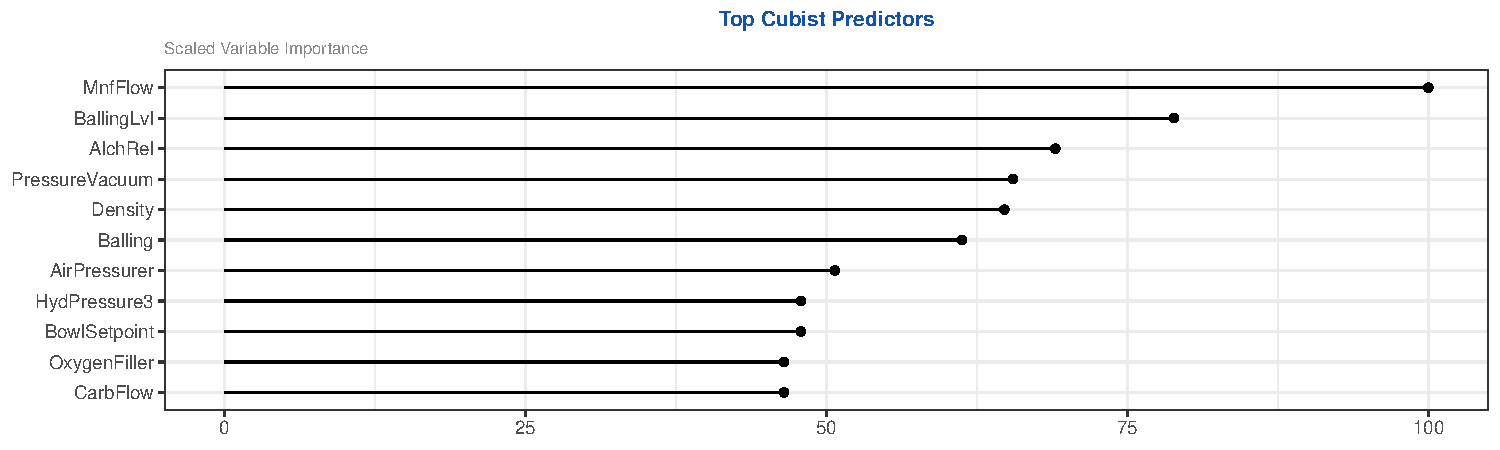
\includegraphics{CONFLICT_Project_Update_files/figure-latex/unnamed-chunk-13-1.pdf}

\hypertarget{conclusion}{%
\chapter{Conclusion}\label{conclusion}}

{[}BETHANY CREATING NEXT STEPS FOR PRODUCTION PROCESS BASED ON FINAL
MODEL{]}

\hypertarget{Appendix}{%
\chapter*{Appendix}\label{Appendix}}
\addcontentsline{toc}{chapter}{Appendix}

\textbf{Code}

\textbf{Data Dictionary}

\textbf{Exploratory Plots and List Models}

\hypertarget{citations}{%
\chapter{Citations}\label{citations}}

Shelton, Robert B. ``PH Values Of Common Drinks.'' Robert B. Shelton,
DDS MAGD Dentist Longview Texas, 2019,
www.sheltondentistry.com/patient-information/ph-values-common-drinks/.

Cubist Model Background: \url{https://www.rulequest.com/cubist-win.html}
Cubist Model Overview:
\url{https://static1.squarespace.com/static/51156277e4b0b8b2ffe11c00/t/56e3056a3c44d8779a61988a/1457718645593/cubist_BRUG.pdf}
Cubist Model Mechanics:
\url{http://ftp.uni-bayreuth.de/math/statlib/R/CRAN/doc/vignettes/caret/caretTrain.pdf}{]}


\end{document}
